% 2009 年江苏卷第 4 题：y=A sin(ωx+φ) 在 [−π,0] 上的图象。
% 来源 PDF：普通高考/2009/2009江苏.pdf
% SHA-256：64e417d45911d88d77c047a419dcc259e7c7dc779c79d20df2092755c96a4501
% 原页：2009江苏.pdf 第 1 页（A3 三栏）第 1 栏，书页码 531。
% 绘制依据：按原页曲线在 [−π,0] 上与 x 轴依次交于 −π、−2π/3、−π/3、0，
%   在 −π/2 处取最大值，在 −5π/6、−π/6 处取最小值；取 A=1、φ=0 绘 y=sin3x。
\begin{tikzpicture}[x=1.15cm, y=1.15cm, semithick, every node/.style={inner sep=1.6pt}]
  \draw[->,>=stealth] (-3.55,0) -- (0.75,0) node[below] {$x$};
  \draw[->,>=stealth] (0,-1.55) -- (0,1.75) node[right] {$y$};

  \draw[domain=-3.14159:0, samples=160, smooth] plot (\x,{sin(3*\x r)});

  \node[below left] at (-3.14159,0) {$-\pi$};
  \node[above] at (-2.42,0.06) {$-\dfrac{2\pi}3$};
  \node[above] at (-0.70,0.06) {$-\dfrac{\pi}3$};
  \node[below right] at (0.06,-0.05) {$O$};
\end{tikzpicture}
